% !TeX TXS-program:compile = txs:///xelatex/[--shell-escape]
% IACR Transactions CLASS DOCUMENTATION
% Written by Gaetan Leurent gaetan.leurent@inria.fr (2016-2018)
%
% To the extent possible under law, the author(s) have dedicated all
% copyright and related and neighboring rights to this software to the
% public domain worldwide. This software is distributed without any
% warranty.
%
% You should have received a copy of the CC0 Public Domain Dedication
% along with this software. If not, see
% <http://creativecommons.org/publicdomain/zero/1.0/>.

\documentclass[preprint]{iacrtrans}
\usepackage[utf8]{inputenc}

\setcounter{tocdepth}{4}

%% VERSION
\newcommand{\version}{v.1.0}


%% TITLE
\title{
  
\includegraphics[width=\columnwidth]{logo_zkEVM.png} \\ \vspace{0.3cm}
  Knowledge Hub \\ \vspace{0.3cm}
  Architecture \\ \vspace{0.3cm}
  Economics - Users Fees \vspace{0.3cm}\\
  \version
}

\institute{}


\usepackage{caption}
\usepackage{subcaption}

% This package controls how hyperlinks are displayed
% https://es.overleaf.com/learn/latex/Hyperlinks
\usepackage{hyperref}
\hypersetup{colorlinks=true,linkcolor={red!80!black},urlcolor={blue!80!black}}

%Multiple columns
\usepackage{multicol}

% Used for super caligraphic font \mathscr{}
\usepackage{mathrsfs}

%This ensures spaces when using ensuremath and no $$ are used to introduce math
\usepackage{xspace}

%%%%%% BEGIN OF CODE HIGHLIGHTING ENVIRONMENTS %%%%%%

%   sudo apt install texlive-latex-extra
%   sudo apt install python-pip
%   pip install pygments
%   pip install pygments-lexer-babylon  #contains JSX
%   pip install pygments-lexer-solidity
%   pip install pygments pygments-lexer-babylon pygments-lexer-solidity


% *** COLOR COMMANDS ***
\definecolor{dblackcolor}{rgb}{0.0,0.0,0.0}
\definecolor{dbluecolor}{rgb}{0.01,0.02,0.5}
\definecolor{dgreencolor}{rgb}{0.2,0.4,0.0}
\definecolor{dgraycolor}{rgb}{0.30,0.3,0.30}
\newcommand{\dblue}{\color{dbluecolor}\bf}
\newcommand{\dred}{\color{dredcolor}\bf}
\newcommand{\dblack}{\color{dblackcolor}\bf}
\definecolor{light-gray}{gray}{0.96} %the shade of grey that stack exchange uses

\usepackage{showexpl}% already includes listings package
\makeatletter
\def\lst@filenamerpl{_\textunderscore $\textdollar}
\makeatother
\lstset{frame=shadowbox, basicstyle=\footnotesize\ttfamily, showstringspaces=false,
rulesepcolor=\color{black}, upquote=true}

\lstdefinestyle{scriptStyle}{
    basicstyle=\footnotesize,% control font of code
    preset=\footnotesize,% adjust font size of output
    numbers=none,
    frame=tlbr,
    pos=r,% want output on rightbackgroundcolor=\color{yellow!30},
    width=0.50\linewidth,
}

\lstdefinestyle{terms}{
    basicstyle=\scriptsize\ttfamily,% control font of code
    preset=\footnotesize,% adjust font size of output
}

\lstdefinestyle{termt}{
    basicstyle=\footnotesize\ttfamily,% control font of code
    preset=\footnotesize,% adjust font size of output
	numbers=none,
}

\lstdefinestyle{verb}{
    basicstyle=\footnotesize,% control font of code
    preset=\footnotesize,% adjust font size of output
    frame=tlbr,
    pos=r,% want output on right
%     backgroundcolor=\color{yellow!30},
    width=0.50\linewidth,
}

\lstdefinestyle{verbs}{
    basicstyle=\scriptsize,% control font of code
    preset=\scriptsize,% adjust font size of output
    frame=tlbr,
    pos=r,% want output on right
%     backgroundcolor=\color{yellow!30},
    width=0.50\linewidth,
}

\lstdefinestyle{verbt}{
    basicstyle=\tiny\ttfamily,% control font of code
    preset=\tiny\ttfamily,% adjust font size of output
    frame=tlbr,
    pos=r,% want output on right
%     backgroundcolor=\color{yellow!30},
    width=0.50\linewidth,
}

%Linter for circom
\usepackage{tcolorbox}
\tcbuselibrary{minted,skins,listings}
\definecolor{mybg}{rgb}{0.96,0.96,0.98}
% \lstset{
% 	backgroundcolor = \color{light-gray},
% 	showtabs = False,
% 	tabsize = 2,
% 	showspaces = False,
% 	showstringspaces = False,
% 	commentstyle = {\ttfamily\color{dgreencolor}},
% 	keywordstyle = {\ttfamily\color{dbluecolor}\bfseries},
% 	stringstyle = {\ttfamily\color{dgraycolor}\bfseries},
% 	language = circom,
% 	basicstyle = {\fontsize{7pt}{7pt}\ttfamily},
% 	aboveskip = 1em,
% 	belowskip = 1em,
% 	numbers = left,%none,
% 	numbersep=5pt,    %space line numbers from code
% 	xleftmargin=2em,
% 	frame=single,	% adds a frame around the code
% 	framexleftmargin=1.7em,
% 	numberstyle=\tiny,%\color{gray}
% 	emph = {proc,retp,endp,local},
% 	emphstyle = {\color{blue}\textbf},
% 	literate =
% 		{<==}{{{\color{dbluecolor}<==}}}2
% 		{==>}{{{\color{dbluecolor}==>{}}}}2
% 		{===}{{{\color{dbluecolor}==={}}}}2
% 		{<--}{{{\color{dbluecolor}<---{}}}}2
% 		{-->}{{{\color{dbluecolor}--->{}}}}2
% 		{*}{{{\color{dbluecolor}*{}}}}2
% }

\lstdefinelanguage{circom}{
	keywords=[1]{signal, input, output, public, <==, ==>, ===}, % generic keywords including crypto operations
  	keywordstyle=[1]\color{blue!70!}\bfseries,
	keywords=[3]{pragma, include},
  	keywordstyle=[3]\color{brown}\bfseries,
	keywords=[4]{for, if, var, else},
	keywordstyle=[4]\color{teal}\bfseries,
	keywords=[5]{template, component},
	keywordstyle=[5]\color{violet}\bfseries,
	identifierstyle=\color{black},
	sensitive=false,
	comment=[l]{//},
	morecomment=[s]{/*}{*/},
	commentstyle=\color{green!40!black}\ttfamily,
	stringstyle=\color{blue}\ttfamily,
%	morestring=[b]',
%	morestring=[b]"
}

\newtcblisting{circom}{
  listing engine=listings,
  colback=mybg,
  colframe=black!70,
  listing only,
  listing options={
    language={circom},
	basicstyle=\footnotesize\ttfamily,
    frame=none,
	numbers=none, %left
	numberstyle=\tiny,
	numbersep=9pt,
	tabsize=2,
	breaklines=true,
	showtabs=false,
	captionpos=b
  },
  left=0.2mm,
  top=0cm,
  bottom=0cm,
  boxrule=0.1mm
}

\newtcblisting{js}{
	listing engine=minted,
	colback=mybg,
	colframe=black!30,
	listing only,
	minted style=tango,
	minted language=js,
	minted options={linenos=false,texcl=true},
	left=0.2mm,
	top=0cm,
	bottom=0cm,
	boxrule=0.1mm
}

\lstdefinelanguage{Pil}{
	keywords=[1]{pol, commit, constant, in, is, connect, public, namespace}, % generic keywords including crypto operations
  keywordstyle=[1]\color{blue!70!}\bfseries,
	keywords=[3]{include}, % modules
  keywordstyle=[3]\color{brown}\bfseries,
	keywords=[4]{},% types; money and time units
	keywordstyle=[4]\color{teal}\bfseries,
	keywords=[5]{field, bool, u32, u16, u8},	% environment variables
	keywordstyle=[5]\color{violet}\bfseries,
	identifierstyle=\color{black},
	sensitive=false,
	comment=[l]{//},
	morecomment=[s]{/*}{*/},
	commentstyle=\color{green!40!black}\ttfamily,
	stringstyle=\color{blue}\ttfamily,
%	morestring=[b]',
%	morestring=[b]"
}

\newtcblisting{pil}{
  listing engine=listings,
  colback=mybg,
  colframe=black!70,
  listing only,
  listing options={
    language={Pil},
	basicstyle=\footnotesize\ttfamily,
    frame=none,
	numbers=none,
	numberstyle=\tiny,
	numbersep=9pt,
	tabsize=2,
	breaklines=true,
	showtabs=false,
	captionpos=b
  },
  left=0.2mm,
  top=0cm,
  bottom=0cm,
  boxrule=0.1mm
}

%%%%%%% END OF CODE HIGHLIGHTING ENVIRONMENTS %%%%%%%

\usepackage{url}
\usepackage{tikz}
\usepackage{graphicx} % Required for including images
\usepackage[font=small,labelfont=bf]{caption}  % Required for specifying captions to tables and figures


%%%%%%%%%%%%%%%%%%% BEGIN OF MACROS %%%%%%%%%%%%%%%%%%%

% Cryptocode: https://github.com/arnomi/cryptocode
\usepackage[
lambda,
operators,
landau, %este es el de bigO
probability,
%sets,
logic, %para or,and...
asymptotics,
keys
]{cryptocode}

% My own procedure blocks to show protocols
\createprocedureblock{mypb}{center, boxed}{}{}{linenumbering}
\createprocedureblock{mypbnonum}{center, boxed}{}{}{}

% Numbering style
\renewcommand{\pclnstyle}[1]{\text{#1}}
\renewcommand{\pclnseparator}{.}

% Hyphen inside mathmode
\mathchardef\mhyphen="2D

% Mathbb
\newcommand{\FF}{\ensuremath{\mathbb{F}}\xspace}
\newcommand{\KK}{\ensuremath{\mathbb{K}}\xspace}
\newcommand{\NN}{\ensuremath{\mathbb{N}}\xspace}
\newcommand{\ZZ}{\ensuremath{\mathbb{Z}}\xspace}

% Mathcal
\newcommand{\A}{\ensuremath{\mathcal{A}}\xspace}
\newcommand{\C}{\ensuremath{\mathcal{C}}\xspace}
\newcommand{\E}{\ensuremath{\mathcal{E}}\xspace}
\newcommand{\F}{\ensuremath{\mathcal{F}}\xspace}
\renewcommand{\H}{\ensuremath{\mathcal{H}}\xspace}
\newcommand{\I}{\ensuremath{\mathcal{I}}\xspace}
\renewcommand{\O}{\ensuremath{\mathcal{O}}\xspace}
\renewcommand{\P}{\ensuremath{\mathcal{P}}\xspace}
\newcommand{\R}{\ensuremath{\mathcal{R}}\xspace}
\renewcommand{\S}{\ensuremath{\mathcal{S}}\xspace}
\newcommand{\T}{\ensuremath{\mathcal{T}}\xspace}
\newcommand{\V}{\ensuremath{\mathcal{V}}\xspace}

% Mathscr
% \newcommand{\PPP}{\ensuremath{\mathscr{P}}\xspace}


% Mathfrak
\newcommand{\afr}{\ensuremath{\mathfrak{a}}\xspace}
\newcommand{\bfr}{\ensuremath{\mathfrak{b}}\xspace}

% Caligraphic Combiantions
\DeclareMathAlphabet{\mathpgoth}{OT1}{pgoth}{m}{n}
\newcommand{\plonk}{\ensuremath{\mathcal{P}\mathfrak{lon}\mathcal{K}}\xspace}
\newcommand{\plookup}{\ensuremath{\mathpgoth{plookup}}\xspace}

% Abbreviations
% \newcommand{\Pp}{\ensuremath{\mathcal{P}_{\textsf{poly}}\xspace}}
\newcommand{\MTR}{\ensuremath{\text{MTR}}\xspace}
\newcommand{\MTP}{\ensuremath{\text{MTP}}\xspace}
\newcommand{\LCC}{\ensuremath{\text{LCC}}\xspace}
\newcommand{\FRI}{\ensuremath{\textsf{F}}\xspace}
\newcommand{\z}{\ensuremath{\overline{z}}\xspace}
\newcommand{\fsel}{\ensuremath{f^{\text{sel}}}\xspace}
\newcommand{\tsel}{\ensuremath{t^{\text{sel}}}\xspace}
\newcommand{\Evals}{\ensuremath{\textsf{Evals}}\xspace}
\newcommand{\pparams}{\ensuremath{\text{pp}}\xspace}
\newcommand{\vparams}{\ensuremath{\text{vp}}\xspace}
\newcommand{\pre}{\ensuremath{\text{pre}}\xspace}
\newcommand{\tr}{\ensuremath{\text{tr}}\xspace}
\newcommand{\otr}{\ensuremath{\overline{\text{P}}}\xspace}
\newcommand{\im}{\ensuremath{\text{im}}\xspace}
\newcommand{\seed}{\ensuremath{\textsf{seed}}\xspace}
\newcommand{\transcript}{\ensuremath{\textsf{transcript}}\xspace}
\newcommand{\AIR}{\ensuremath{\textsf{A}}\xspace}
\newcommand{\eAIR}{\ensuremath{\textsf{eA}}\xspace}
\newcommand{\accept}{\ensuremath{\textsf{accept}}\xspace}
\newcommand{\reject}{\ensuremath{\textsf{reject}}\xspace}
\newcommand{\eFRI}{\ensuremath{\epsilon_{\textsf{FRI}}}\xspace}
\newcommand{\eSTARK}{\ensuremath{\epsilon_{\textsf{STARK}}}\xspace}
\newcommand{\eeSTARK}{\ensuremath{\epsilon_{\textsf{eSTARK}}}\xspace}
\newcommand{\eC}{\ensuremath{\epsilon_{\textsf{C}}}\xspace}
\newcommand{\ePlo}{\ensuremath{\epsilon_{\textsf{Plo}}}\xspace}
\newcommand{\eMulEq}{\ensuremath{\epsilon_{\textsf{MulEq}}}\xspace}
\newcommand{\eCon}{\ensuremath{\epsilon_{\textsf{Con}}}\xspace}
\newcommand{\eArgs}{\ensuremath{\epsilon_{\textsf{Args}}}\xspace}
\newcommand{\RS}{\ensuremath{\textsf{RS}[\FF,H,\rho]}\xspace}
\newcommand{\RSK}{\ensuremath{\textsf{RS}[\KK,H,\rho]}\xspace}
\newcommand{\LH}{\ensuremath{\textsf{LH}}\xspace}
\newcommand{\ID}{\ensuremath{\textsf{ID}}\xspace}

% C12
\newcommand{\POSEIDON}{\ensuremath{\texttt{POSEIDON12}}\xspace}
\newcommand{\acode}{\ensuremath{\texttt{a}}\xspace}
\newcommand{\CONST}{\ensuremath{\texttt{C}}\xspace}
\newcommand{\PARTIAL}{\ensuremath{\texttt{PARTIAL}}\xspace}
\newcommand{\CMULADD}{\ensuremath{\texttt{CMULADD}}\xspace}
\newcommand{\EVPOL}{\ensuremath{\texttt{EVPOL4}}\xspace}
\newcommand{\FFT}{\ensuremath{\texttt{FFT4}}\xspace}
\newcommand{\nextStep}{\ensuremath{\textsf{'}}\xspace}
\newcommand{\scale}{\ensuremath{\texttt{s}}\xspace}
\newcommand{\firstW}{\ensuremath{\texttt{firstW}}\xspace}
\newcommand{\firstWSquare}{\ensuremath{\texttt{firstW2}}\xspace}
\newcommand{\incW}{\ensuremath{\texttt{incW}}\xspace}
% Caligraphic Combiantions
 \DeclareMathAlphabet{\mathpgoth}{OT1}{pgoth}{m}{n}

% Abbreviations
\newcommand{\stoc}{\texttt{S2C}\xspace}
\newcommand{\ctos}{\texttt{C2S}\xspace}


% Make a nice emptyset
\let\oldemptyset\emptyset
\let\emptyset\varnothing

% Make a nice phi and epsilon
\let\oldphi\phi
\let\phi\varphi
\let\oldepsilon\epsilon
\let\epsilon\varepsilon

% Make a nice q.e.d. symbol
\renewcommand\qedsymbol{\ensuremath{\blacksquare}\xspace}

\theoremstyle{definition}
\newtheorem{protocol}{Protocol}
\newtheorem{bremark}{Remark}

\usepackage{paralist} % for compactitem environment

%%%%%%%%%%%%%%%%%%% END OF MACROS %%%%%%%%%%%%%%%%%%%

% \begin{pcvstack}[boxed, center]
% % \pcsetargs{codesize=\scriptsize{}}

% \procedure{}{
%   \textbf{Prover } \P(g_1(x))  \< \< \textbf{verifier } \V(g_1(x)) \\[][\hline]
%   \< \sendmessageright{top={$f_1(s)$, $f_2(s)$}} \< \\[-2mm]
%   \< \sendmessageleft{top={randomness}} \< \\[-2mm]
%   \< \sendmessageright{top={$f_3(s)$}} \< \\[-2mm]
%   \< \< \text{Samples a random } z \in \FF \text{ and computes } z\vec{g}. \\[-2mm]
%   \< \sendmessageleft{top={$z$}} \< \\[-2mm]
%   \text{Computes evaluations:} \< \< \\
%   \t g_1(z), f_1(z), f_2(z), f_3(z) \< \< \\[-2mm]
%   \< \sendmessageright{top={$g_1(z)$, $f_1(z)$, $f_2(z)$, $f_3(z)$}} \< \\[-2mm]
%   \< \sendmessageleft{top={$v$}} \< \\[-2mm]
%   \< \sendmessageright{top={$\pi$}} \< \\[-2mm]
%   \< \< \text{Verifies the opening proof } \pi \text{ and checks that:} \\
%   \< \< \t g_1(z)(f_1(z) + f_2(z)) - f_3(z) = 0
% }
% \end{pcvstack}

\newcommand{\definedir}[2]{\newcommand{#1}{#2}}
\definedir{\topicdir}{..}
\definedir{\zkevmdir}{../../../..}


\begin{document}
\begin{titlepage}
\centering
\maketitle
\today
\end{titlepage}

% use optional argument because the \LaTeX command breaks the PDF keywords
% \keywords[\publname, ToSC, TCHES, LaTeX]{TBD \and TBD}

%{\hypersetup{linkcolor=.}\tableofcontents}

\newpage
% !TeX spellcheck = en_US
% !TeX root = ../build/users-fees.tex
% !TeX TXS-program:compile = txs:///xelatex/[--shell-escape]



\section{Basic Ethereum Fee Schema}

Before explaining the user fee schema followed in the zkEVM, let us devote this section to explain how the basic Ethereum fee schema works. Recall that the \textbf{Gas} is a unit that accounts the resources used when processing a transaction. \textbf{At the time of sending a transaction}, users have to define two parameters that will determine the fee imposed on them:

\begin{enumerate}
\item \texttt{gasLimit}: This parameter represents the upper limit of gas units that a user authorizes for consumption during the transaction.

\item \texttt{gasPrice}: It refers to the amount of Wei a user is willing to pay per unit of gas for the transaction execution. Trying to be more concrete, there exists a dynamic market interaction between users and network nodes. In Ethereum ecosystem, if a user desires to expedite the processing of their transaction, they must adjust the \texttt{gasPrice} accordingly. Essentially, a higher \texttt{gasPrice} becomes an incentive for network nodes to prioritize the associated transaction.

\end{enumerate}

At the \textbf{start of the transaction processing}, the following
amount of Wei is subtracted from the source account balance:
\[
\texttt{gasLimit} \cdot \texttt{gasPrice}.
\]
Then, when the processing of the transaction is finished, if $\texttt{gasUsed} > \texttt{gasLimit}$, the transaction is reverted. Otherwise, the amount of Wei associated with the unused gas is refunded. The refunded amount of Wei that is added back to the source account is calculated as:
\[
\texttt{gasLimit} \cdot \texttt{gasPrice} - \texttt{gasUsed} \cdot \texttt{gasPrice}.
\]

For reasons that will arise at the last section of this document, it is important to observe that when the transaction is being processed, the balance of the source account during transaction processing differs from its state at the time of sending the transaction. More specifically, if the \texttt{BALANCE} opcode is invoked during the transaction processing, the output will be
\[
\texttt{initialBalance} - \texttt{gasLimit} \cdot \texttt{gasPrice},
\]
where \texttt{initialBalance} represents the balance of the source account before the execution of the transaction.






%%%%%%%%%%%%%%%%%%%%%%%%%%%%%%%%%%%%%%%%%%%%%%%%%%%%%%%%%%%%%%%%%%%%%%%%%%%%%%%%
\section{Generic User Fee Strategy of Layer 2 Solutions}

In general, Layer 2 solutions adopt a fee strategy wherein the L2 gas price is a percentage of the L1 gas price. This approach aligns with the goal of making transactions less costly for the user. Using this approach, we can define \texttt{L2GasPrice} as follows:
\[
\texttt{L2GasPrice} = \texttt{L1GasPrice} \cdot \texttt{L1GasPriceFactor}.
\]
where \texttt{L1GasPrice} denotes the network variable indicating the minimum gas price required to sign a transaction, and $0 < \texttt{L1GasPriceFactor} < 1$ defines the reduction factor. For example, let us suppose that Layer 1 is accepting transactions having a signed gas price of $20$ GWei, so $\texttt{L1GasPrice} = 20$ and that L2 gas price is reduced a $96\%$. Then:
\begin{gather*}
\texttt{L1GasPrice} = 20 \text{ GWei} \text{ and } \texttt{L1GasPriceFactor} = 0.04 \ (4\% \text{ of L1 } \texttt{gasPrice}) \\
\text{therefore, } \texttt{L2GasPrice} = 20 \text{ GWei} \cdot 0.04 =  0.8 \text{ GWei}
\end{gather*}

You can check the current fees at \url{https://l2fees.info}. However, this is not as easy as it may seem and there are additional aspects to consider:

\begin{enumerate}[a)]
\item The gas price on L1 is subject to fluctuations over time (See Figure \ref{fig:refresh-gas-prices}). How does the zkEVM transaction processing mechanism account for these variations?

\item As we have said before, when initiating a transaction on Layer 1, increasing the gas price can serve to prioritize transactions. How does the Layer 2 solution effectively manage these priorities?

\item The Gas schema on Layer 1 may not necessarily align with the actual resources expended by the Layer 2 solution. How does the L2 solution address and reconcile any discrepancies between the L1 gas schema and the real resource utilization on L2?

\end{enumerate}

\begin{figure}[H]
\centering
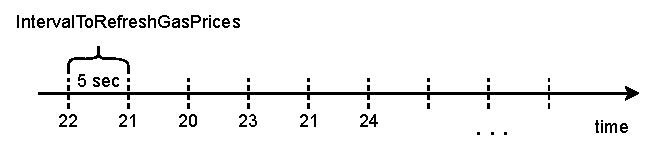
\includegraphics[width=0.8\columnwidth]{\zkevmdir/figures/architecture/economics-users-fees/l1-gasprice-refresh.drawio}
\caption{Observe that L1 gas prices, refreshed every $5$ seconds (which can be changed modifying a configuration parameter called \texttt{IntervalToRefreshGasPrices}) fluctuate over time.}
\label{fig:refresh-gas-prices}
\end{figure}

In the following sections, we will thoroughly examine the significance of fees in Layer 2 and provide detailed answers to the previously mentioned questions.

We will now delve into the initial phase of the process (see Figure \ref{fig:rpc}), which involves the \textbf{RPC} component of zkEVM. This phase spans from the moment the user submits the transaction, the price is estimated through a pre-execution of the transaction, to the final decision of storing it in the \textbf{Pool} or rejecting it based on a set of conditions.

\begin{figure}[H]
\centering
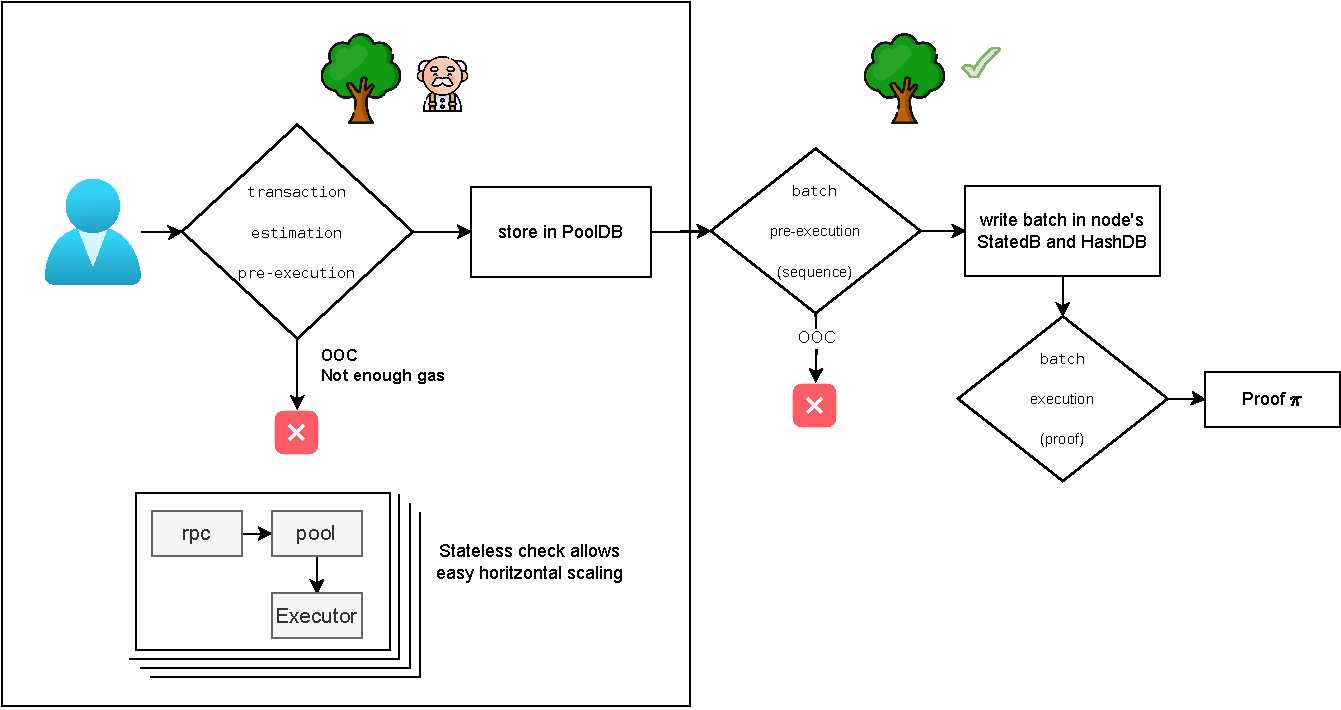
\includegraphics[width=0.8\columnwidth]{\zkevmdir/figures/architecture/economics-users-fees/rpc-preexecution.drawio}
\caption{Illustration of the first phase in the zkEVM flow, involving the \textbf{RPC} component, from user transaction submission to pre-execution to estimate optimal pricing and potential storage in the \textbf{Pool} or rejection.}
\label{fig:rpc}
\end{figure}







%%%%%%%%%%%%%%%%%%%%%%%%%%%%%%%%%%%%%%%%%%%%%%%%%%%%%%%%%%%%%%%%%%%%%%%%%%%%%%%%
\section{Gas Price Suggester}

This section will be devoted to constructing a scheme for the user to send a transaction to the zkEVM in such a way that their user experience is maximized. We will present different attempts, each addressing a problem from the previous one.

\subsection{Naive Approach}

Consider a scenario in which a user intends to send a transaction on Layer 2. However, the user lacks information regarding the appropriate gas price he/she has to sign with its transaction. Consequently, the user asks via RPC for a suggestion of the current gas price to sign with, as shown in Figure \ref{fig:suggest-l2-gas-price}. The suggested price will be \texttt{L2GasPrice}, which recall that is computed the following way:
\[
\texttt{L2GasPrice} = \texttt{L1GasPrice} \cdot \texttt{L1GasPriceFactor}.
\]
\begin{figure}[H]
\centering
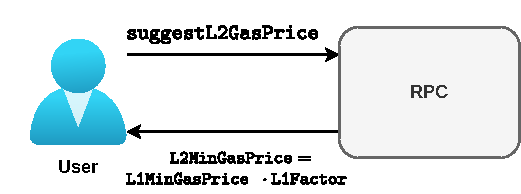
\includegraphics[scale=0.7]{\zkevmdir/figures/architecture/economics-users-fees/suggest-gasprice.drawio}
\caption{The user asks RPC for the suggested gas price.}
\label{fig:suggest-l2-gas-price}
\end{figure}

Now that the user knows a suggestion for the gas price he/she has to include, the user sends the desired L2 transaction with a choice of gas price that we will call \textbf{signed gas price}, denoted as \texttt{GasPriceSigned}. Observe that this choice can be  equal to, greater than, or lower than the suggested price, each resulting in distinct scenarios: either the acceptance or rejection of the transaction, as illustrated in Figure \ref{fig:send-tx}. We will delve on this later on.
\begin{figure}[H]
\centering
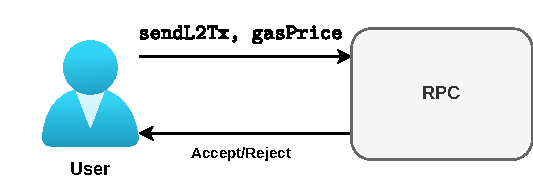
\includegraphics[scale=0.7]{\zkevmdir/figures/architecture/economics-users-fees/send-l2-tx-gasprice.drawio}
\caption{The user sends a transaction with the decided \texttt{GasPriceSigned} to RPC, a decision is taken on whether to accept or reject it.}
\label{fig:send-tx}
\end{figure}

In case the \texttt{GasPriceSigned} decided by the user is less than the current \texttt{L2GasPrice}, the transaction is automatically rejected and not included into the pool. This error is named \texttt{ErrGasPrice}.

\subsection{Decision Interval Approach}

\paragraph*{Problematic}

The previous framework has a limitation as there is a time gap between asking for a suggested gas price and sending the transaction in which the gas price can fluctuate. This fact leads the unwanted situation depicted in Figure \ref{fig:bad-ux}:
\begin{figure}[H]
\centering
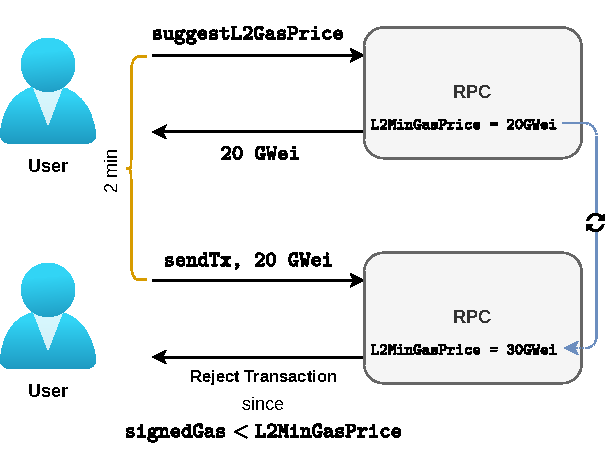
\includegraphics[scale=0.7]{\zkevmdir/figures/architecture/economics-users-fees/fees-bad-ux.drawio}
\caption{The user asks for a suggested price, the current suggested gas price is of $20$ GWei and decides to sign $20$ GWei, but when he sends the transaction the suggested gas price has increased to $30$ GWei and the transaction is rejected. }
\label{fig:bad-ux}
\end{figure}

In Figure \ref{fig:bad-ux} we can observe that although the user has sent a gas price according to the suggested price, after the time lapse between one step and the other, the price has increased and the transaction is rejected.

\paragraph*{Solution}

The \textbf{solution} is to give a user some period of time in order to make the choice and sending the transaction. More specifically, we give a margin of $5$ minutes (controlled by the \texttt{MinAllowedGasPriceInterval} parameter). The \texttt{MinL2GasPrice} is defined as the minumum suggested gas price of $5$ minutes before sending the transaction refreshed every $5$ seconds (controlled by the \texttt{IntervalToRefreshGasPrices} parameter). If the signed gas price does not strictly exceed \texttt{MinL2GasPrice},
\[
\texttt{GasPriceSigned} > \texttt{L2MinGasPrice},
\]
we automatically \textbf{reject} the transaction, since it will not be possible to cover costs. Figure \ref{fig:minimum-gas-price} depicts an example on how \texttt{MinL2GasPrice} is computed, which in this precise case is $18$ GWei.

\begin{figure}[H]
\centering
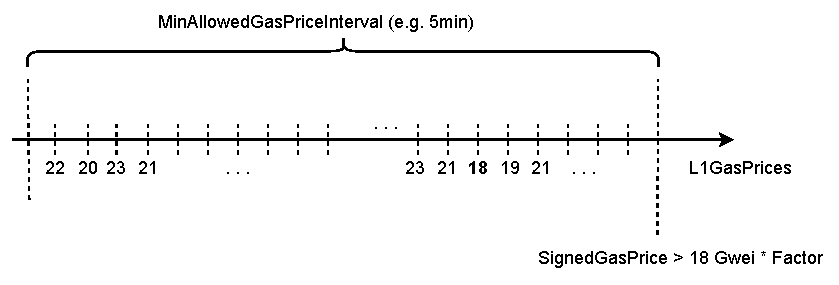
\includegraphics[scale=0.7]{\zkevmdir/figures/architecture/economics-users-fees/min-allowed-price-interval.drawio}
\caption{Timeline displaying the current \texttt{L1GasPrice} and its associated suggested gas price. In this case \texttt{MinL2GasPrice}=$18$. }
\label{fig:minimum-gas-price}
\end{figure}

This previous parameters can be configured in the Polygon zkEVM node configuration files. More specifically, it can be configures in the \texttt{[Pool]} section of the configuration TOML, which can be found \href{https://github.com/0xPolygonHermez/zkevm-node/blob/b938572f138ba6cc40ef6736153c469afeb11c96/config/default.go#L37}{here}.

\vspace{1em}

\begin{toml}
[Pool]
...
DefaultMinGasPriceAllowed = 0
MinAllowedGasPriceInterval = "5m"
PollMinAllowedGasPriceInterval = "1s"
IntervalToRefreshGasPrices = "5s"
...
\end{toml}

%TODO Marc: Review and extend.
%Where the meaning of the parameters is:
%
%\begin{itemize}
%\item \texttt{DefaultMinGasPriceAllowed:} It is the default min gas price to suggest.
%\item \texttt{MinAllowedGasPriceInterval:} It is the interval to look back of the suggested min gas price for a transaction.
%\item \texttt{PollMinAllowedGasPriceInterval:} It is the interval to poll L1 to find the suggested L2 min gas price.
%\item \texttt{IntervalToRefreshGasPrices:} It is the interval to refresh L2 gas prices.
%\end{itemize}
%
%When computing the L1 \texttt{gasPrice}, we can activate the \texttt{multigasprovider}, which allows using multiples sources for computing the L1 \texttt{gasPrice}:
%\begin{toml}
%[Etherman]
%...MultiGasProvider = false
%\end{toml}
%
%\vspace{10 mm}


\subsection{Final Approach}

\paragraph*{Problematic}

However, in the previous design, the zkEVM endpoint responsible for offering a gas price suggestion to the user, known as \textbf{L2 Gas Price Suggester}, faces a significant problem design. The price of posting transactional data to L1 is charged to the zkEVM network to the \textbf{full L1 price}. Therefore, if we propose a gas price using \texttt{L1GasPriceFactor}, representing the measure of computational reduction in L2, there is a risk of running out of Wei reserves for posting data to L1.

\paragraph*{Solution}

In order to solve the previous situation, we will recommend a slightly higher percentage of the gas price to the user, employing a \texttt{SuggesterFactor} of $0.15 \approx 4 \cdot \texttt{L1GasPriceFactor}$:
\[
\texttt{GasPriceSuggested} = \texttt{L1GasPrice} \cdot \texttt{SuggestedFactor}.
\]


\subsection{Numerical Example: \texttt{L2MinGasPrice}}


In Figure \ref{fig:numerical-example} we can observe that when the user queries the suggested gas price through the RPC, the network responds the current suggested gas price computed as $0.15 \cdot 19 = 2.85$, where $19$ is the current L1 gas price, updated every $5$ seconds. Observe that, using the naive approach, the user should have signed for a gas price strictly higher than $3.15$, since the L1 gas price at the moment of sending the transaction is $21$. However, using the final approach, at the time of sending the transaction, the RPC will accept the transaction as long as $\texttt{GasPriceSigned}$ is strictly higher than the minimum suggested gas price from the 5 minutes interval (highlighted in \textbf{bold} in the figure), which in this instance is $19 \cdot 0.15 = 2.85$. In order to get his transaction accepted, the user sets the gas price of the transaction to $\texttt{GasPriceSigned} = 3.3 > 2.85 = \texttt{L2MinGasPrice}.$ The user has signed at a higher gas price than the suggested to ensure that the transaction is executed and maybe prioritize it among others.


\begin{figure}[H]
\centering
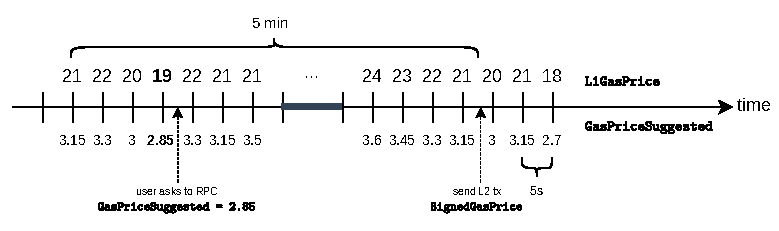
\includegraphics[scale=1]{\zkevmdir/figures/architecture/economics-users-fees/example-minimum-gas-price.drawio}
\caption{The user asks for a \texttt{GasPriceSuggested} = $2.85$ and decides to set \texttt{SignedGasPrice} = $3.3$ to ensure that the transaction is executed.}
\label{fig:numerical-example}
\end{figure}





%%%%%%%%%%%%%%%%%%%%%%%%%%%%%%%%%%%%%%%%%%%%%%%%%%%%%%%%%%%%%%%%%%%%%%%%%%%%%%%%
\section{Dealing with L1/L2 Cost Discrepancies}

\subsection{Cost Discrepancies Challenges}

As we have said before, in Ethereum, \textbf{gas} accounts for the resources used by a transaction. In particular, it takes into account two elements in particular: the \textbf{data availability}, that is, the transactions bytes and the \textbf{processing resources}, like CPU, Memory and Storage. A notable challenge arises when certain operations consume low gas in Layer 1 but represent a major cost in Layer 2. In other words, the reduction factor expressed in the L1-L2 gas price relationship
\[
\texttt{L2GasPrice} = \texttt{L1GasPrice} \cdot \texttt{L1GasPriceFactor}
\]
may not be constant among all the computational resources, introducing a problem.

L2 execution costs are variable, depending on the state of the transaction and typically offer a smaller cost per gas. However, the costs associated with data availability are fixed once the transaction is known, and they are directly proportional to L1 data availability costs. Consequently, in our pricing schema, L2 transactions with high data availability costs and small execution costs are a significant challenge. This presents another pricing misalignment issue we need to face.

\subsection{Possible Solutions}

Recall that the Ethereum fee in L1 is computed as
\[
\texttt{gasUsed} \cdot \texttt{gasPrice},
\]
giving us two ways of solving the misalignment problem between costs in L1 and L2:

\begin{enumerate}[(A)]
\item \textbf{Arbitrum Approach. Increase \texttt{gasUsed}. }
This approach involves modifying the gas schema to elevate the Gas costs associated with data availability. While this strategy is relatively straightforward to implement and comprehend, it comes with a notable implication: \textbf{it changes the Ethereum protocol}. An L1 Ethereum transaction may execute different when compared to the same transaction executed in L2.

\item \textbf{Effective Gas Price Approach. Increase \texttt{gasPrice}. }
If we aim to avoid modifying the gas, the alternative is to increase the gas price to cover the costs. Unlike the previous approach, this doesn't alter the Ethereum specifications. However, determining a fair gas price becomes a complex task. Moreover, we have to take into account that L2 users should be able to prioritize its transactions also increasing gas price, as they are used to. \textbf{This is actually our approach.}
\end{enumerate}


\subsection{Effective Gas Price Approach}

We will now develop how the \textbf{Effective Gas Price Approach} works. First, the user signs a relatively high gas price at the time of sending the L2 transaction. Later on, by pre-executing the sent transaction, the \textbf{sequencer} establishes a fair gas price according to the amount of resources used. To do so, the \textbf{sequencer} provides an \texttt{EffectivePercentage}, which represents the portion of the total charged to the user. In other words, this percentage will be used in order to compute the factor of the signed transaction's signed gas price which should be refunded to the user.

To calculate the \texttt{EffectivePercentage}, one option is to consider the pricing resources based on the number of \textbf{consumed counters} within our proving system. However, understanding this metric can be challenging for users because stating the efficiency through counters is not intuitive at the time of prioritizing their transactions. As we want to prioritize a positive user experience, we will consider an alternative where gas is used for calculations, as it is more user-friendly. So, our primary objective is to compute \texttt{EffectivePercentage} exclusively using gas, allowing users to prioritize their transactions through the use of gas price without the need for intricate counter-based considerations. The effective percentage is computes as follows:
\[
\texttt{EffectivePercentage} = \frac{\texttt{GasPriceFinal}}{\texttt{GasPriceSigned}}.
\]
Observe that, by modifying \texttt{GasPriceFinal}, which is the gas price charged at the end of the whole processing by the sequencer, we can modify the amount of Wei that we will charge to the user in order to process the sent transaction.

To send this percentage, the \textbf{sequencer} provides a single byte \texttt{EffectivePercentageByte} $\in \{0, 1, \dots, 255 \}$, which is computed from the \texttt{EffectivePercentage}:
%TODO: Review this formula
\[
\texttt{EffectivePercentageByte} = (\texttt{EffectivePercentage}\cdot 256) - 1.
\]

As having \texttt{EffectivePercentage} implies having \texttt{EffectivePercentageByte}, and vice versa, we will abuse of notation and use them interchangeably as \texttt{EffectivePercentage}. For example, setting an \texttt{EffectivePercentageByte} of $255 (= \texttt{0xFF})$ would mean that the \texttt{EffectivePercentage} = $1$ so user would pay the totality of the gas price signed when sending the transaction:
\[
\texttt{GasPriceFinal} = \texttt{GasPriceSigned}.
\]

In contrast, setting \texttt{EffectivePercentageByte} to $127$ would mean that
\[
\texttt{EffectivePercentage} = 0.5
\]
so it will reduce the gas price signed by the user to the half:
\[
\texttt{GasPriceFinal} = \frac{\texttt{GasPriceSigned}}{2}.
\]
This implies that the user will be refunded half of the price he initially signed for. Observe that, in this schema, users \textbf{must trust the sequencer}.





%%%%%%%%%%%%%%%%%%%%%%%%%%%%%%%%%%%%%%%%%%%%%%%%%%%%%%%%%%%%%%%%%%%%%%%%%%%%%%%%
\section{Introducing \texttt{BreakEvenGasPrice}}

As service providers, our primary goal is to \textbf{avoid accepting transactions that result in financial losses}. To attain this objective, we will determine the \texttt{BreakEvenGasPrice}, representing the lowest gas price at which we do not incur losses. As explained before, we will split the computation in two to take into account differently costs associated with data availability and costs associated with processing resources.
%TODO he canviat el final de la frase q posava: costs associated with used gas


\subsection{Costs Associated with Data Availability}

Costs associated with Data Availability will be computed as
\[
\texttt{DataCost} \cdot \texttt{L1GasPrice},
\]
where \texttt{DataCost} is the cost in Gas for data in L1.

In the Ethereum ecosystem, the cost of data varies depending on whether it involves zero bytes or non-zero bytes. In particular, \textbf{non-zero bytes} cost \textbf{$16$ Gas} meanwhile \textbf{zero bytes} \textbf{$4$ Gas}. Also recall that, when computing non-zero bytes cost we should take into account some constant data always appearing in a transaction and are not included in the RLP: the signature, consisting on $65$ bytes and the previously defined \texttt{EffectivePercentageByte}, which consists in a single byte. This results in a total of $66$ constantly present bytes.

Taking all in consideration, \texttt{DataCost} can be computed as:
\begin{gather*}
\texttt{DataCost} = \underbrace{(\texttt{TxConstBytes} + \texttt{TxNonZeroBytes}) \cdot \texttt{NonZeroByteGasCost}}_\text{Non Zero Bytes} \\
+ \underbrace{\texttt{TxZeroBytes} \cdot \texttt{ZeroByteGasCost}}_\text{Zero Bytes}
\end{gather*}
where \texttt{TxZeroBytes} (respectively \texttt{TxNonZeroBytes}) represents the count of zero bytes (respectively non-zero bytes) in the raw transaction sent by the user.


\subsection{Computational Costs}

For the computational cost, we will use the following formula:
\[
\texttt{GasUsed} \cdot \texttt{L2GasPrice},
\]
where recall that we can obtain \texttt{L2GasPrice} by multiplying \texttt{L1GasPrice} by chosen factor less than $1$
\[
\texttt{L2GasPrice} = \texttt{L1GasPrice} \cdot \texttt{L1GasPriceFactor}.
\]
In particular, we will choose a factor of $0.04$.

In contrast to data availability costs, to compute computational costs we will need to \textbf{execute} the transaction.

\subsection{Total Price of the Transaction}

Combining both \textbf{data} and \textbf{computational} costs, we will refer to it as \texttt{TotalTxPrice}:
\[
\texttt{TotalTxPrice} = \underbrace{\texttt{DataCost} \cdot \texttt{L1GasPrice}}_\text{Data availability cost} + \underbrace{\texttt{GasUsed} \cdot \texttt{L1GasPrice} \cdot \texttt{L1GasPriceFactor}}_\text{Computational cost}
\]

To establish the gas price at which the total transaction cost is covered we can compute \texttt{BreakEvenGasPrice} as the following ratio:
\[
\texttt{BreakEvenGasPrice} = \frac{\texttt{TotalTxPrice}}{\texttt{GasUsed}}.
\]
Additionally, we incorporate a factor $\texttt{NetProfit} \geq 1$ that allows us to achieve a slight profit margin:
\[
\texttt{BreakEvenGasPrice} = \frac{\texttt{TotalTxPrice}}{\texttt{GasUsed}} \cdot \texttt{NetProfit}.
\]

We could now conclude that if
\[
\texttt{SignedGasPrice} > \texttt{BreakEvenGasPrice}
\]
it is supposed to be financially safe to accept the transaction. But at this point the following problem arises: in the RPC component, we're only pre-executing the transaction, meaning we're using an incorrect state root. Consequently, the \texttt{GasUsed} is only an approximation. This implies that we need to multiply the result by a chosen factor before comparing it to the signed price. This ensures that the costs are covered in case more gas is ultimately required to execute the transaction. This factor is named \texttt{BreakEvenFactor}. Now we can conclude that if:
\[
\texttt{SignedGasPrice} > \texttt{BreakEvenGasPrice} \cdot \texttt{BreakEvenFactor}
\]
it is safe to accept the transaction.

Observe that we still need to introduce gas price prioritization, which will be covered later on.


\subsection{Numerical Example: Computing \texttt{BreakEvenGasPrice}}

Recall the example proposed before, where the \texttt{GasPriceSuggested} provided by RPC was $2.85$ GWei/Gas but the user ended up by setting \texttt{GasPriceSigned} to $3.3$. Figure \ref{fig:numerical-example-break-even-gas-price} depicts the current situation.

\begin{figure}[H]
\centering
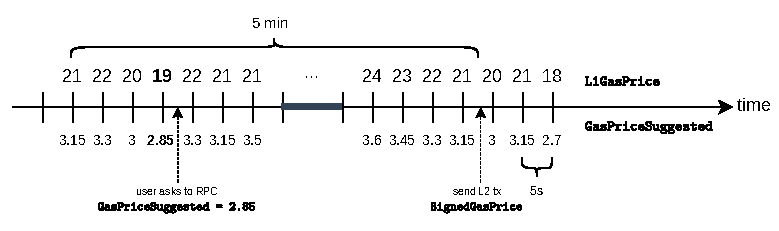
\includegraphics[scale=0.9]{\zkevmdir/figures/architecture/economics-users-fees/example-minimum-gas-price.drawio}
\caption{Timeline displaying the current \texttt{L1GasPrice} and its associated suggested gas price.}
\label{fig:numerical-example-break-even-gas-price}
\end{figure}

Suppose the user sends a transaction having: $200$ non-zero bytes, including the constant ones and $100$ zero bytes. Moreover, at the time of pre-executing the transaction, which is done without getting an \textbf{OOC} error, $60,000$ Gas is consumed. Recall that, since we are using a \textbf{wrong} state root, this gas is only an estimation. Hence, following the formulas previously explained, the total transaction cost is of
\begin{gather*}
\texttt{TotalTxPrice} = \texttt{DataCost} \cdot \texttt{L1GasPrice} + \texttt{GasUsed} \cdot \texttt{L1GasPrice} \cdot \texttt{L1GasPriceFactor} \Rightarrow \\
\texttt{TotalTxPrice} = \left( 200 \cdot 16 + 100 \cdot 4 \right) \cdot 21 + 60,000 \cdot 21 \cdot 0.04 = 126,000 \text{ GWei}.
\end{gather*}

Observe that $21$ appearing in the substitution is the \texttt{L1GasPrice} at the time of sending the transaction.

Now, we are able to compute the \texttt{BreakEvenGasPrice} as
\[
\texttt{BreakEvenGasPrice} = \frac{\texttt{TotalTxPrice}}{\texttt{GasUsed}} = \frac{126,000 \text{ GWei}}{60,000 \text{ Gas}} \cdot 1,2 = 2.52 \text{ GWei/Gas}.
\]

We have introduced a \texttt{NetProfit} value of $1.2$, indicating a target of a $20\%$ gain in this process. At a first glance, we might conclude acceptance since $\texttt{GasPriceSigned} = 3.3 > 2.52$ but, recall that this is only an estimation, gas consumed with the correct state root can differ. To avoid this issue, we introduce a \texttt{BreakEvenFactor} of $30\%$ to account for estimation uncertainties:
\[
\texttt{GasPriceSigned} = 3.3 > 3.276 = 2.52 \cdot 1.3 = \texttt{BreakEvenGasPrice} \cdot \texttt{BreakEvenFactor}.
\]

Consequently, we decide to \textbf{accept the transaction}.


\subsection{Numerical Example: Importance of \texttt{BreakEvenFactor}}

Imagine we disable the \texttt{BreakEvenFactor} setting it to $1$. Our original transaction's pre-execution consumed $60,000$ Gas
\[
\texttt{GasUsedRPC} = 60,000.
\]

However, imagine that the correct execution at the time of sequencing consumes $35,000$ Gas. If we recompute \texttt{BreakEvenGasPrice} using this updated used gas, we get $3.6 \text{GWei/Gas}$, which is way higher than the original one. That means that, we should have charged the user with a higher gas price in order to cover the whole transaction cost, which now is of $105,000$ GWei.

But, since we are accepting all the transactions signing more than $2.85$ of gas price, we do not have margin to increase more. In the worst case we are loosing
\[
105,000 - 35,000 \cdot 2.85 = 5,250 \text{ GWei}.
\]

Introducing \texttt{BreakEvenFactor} we are limiting the accepted transactions to the ones having
\[
\texttt{GasPriceSigned} \geq 3.27,
\]
in order to compensate such losses.

In this case, we have the flexibility to avoid losses and adjust both user and our benefits since
\[
105,000 - 35,000 \cdot 3.27 < 0.
\]

\paragraph*{Final Note}
In the example, even though we assumed that the decrease in \texttt{BreakEvenGasPrice} is a result of executing with a correct state root, it can also decrease significantly due to a substantial reduction in \texttt{L1GasPrice}.





\section{\texttt{EffectiveGasPrice}: Introducing Priority}

Prioritization of transactions in Ethereum is determined by \texttt{GasPriceSigned}: transactions signed at a higher price will be given priority. To implement this, consider that users are only aware of two gas price values: the one signed with the transaction, called \texttt{GasPriceSigned} and the current \texttt{GasPriceSuggested}, which is the one that provides the RPC. 

It is important to note that this part of the process \textbf{is not} computed in the \textbf{RPC} but in the \textbf{Sequencer}, so it possible that the suggested gas price at this moment differs from the suggested one when user sent the transaction.

At the time of sequencing a transaction, we should prioritize ones among the others, depending basically on both \texttt{GasPriceSigned} and current \texttt{GasPriceSuggested}. In the case that $\texttt{GasPriceSigned} > \texttt{GasPriceSuggested}$, we establish a priority ratio as follows:
\[
\texttt{PriorityRatio} = \frac{\texttt{GasPriceSigned}}{\texttt{GasPriceSuggested}} - 1.
\]

If $\texttt{GasPriceSigned} \leq \texttt{GasPriceSuggested}$, the user has chosen not to prioritize its transaction, and maybe we can reject the transaction due to low gas price. In this case, we establish a priority ratio to be $0$.

Finally, the \texttt{EffectiveGasPrice} will be computed as:
\[
\texttt{EffectiveGasPrice} = \texttt{BreakEvenGasPrice} \cdot (1 + \texttt{PriorityRatio}).
\]


\subsection{Numerical Example: Priority}

 Let's see it with an example. Recall that, in the previous example, we were signing a gas price of $3.3$ at the time of sending the transaction. Suppose that, at the time of sequencing a transaction, the suggested gas price is 3:
\[
\texttt{GasPriceSigned} = 3.3, \quad \texttt{GasPriceSuggested} = 3.
\]
The difference between both is taken into account in the priority ratio:
\[
\texttt{PriorityRatio} = \frac{3.3}{3} - 1 = 0.1.
\]
Henceforth, the estimated \texttt{EffectiveGasPrice} (that is, the one using the RPC gas usage estimations) will be
\[
\texttt{EffectiveGasPrice} = 2.52 \cdot (1 + 0.1) = 2.772 \text{ GWei/Gas}.
\]

% !TeX spellcheck = en_US
% !TeX root = ../build/users-fees.tex
% !TeX TXS-program:compile = txs:///xelatex/[--shell-escape]



\section{User Fees Flows}

In this section, we will delve into the economic process that starts when a user wants to send some transaction to the L2 network. Our discussion will be split into two parts: firstly, the transaction flow done by the \textbf{RPC} until it is dispatched by the user, concluding when it is stored in the \textbf{Pool}. Secondly, we will examine the sequence transaction flow managed by the \textbf{Sequencer}, ending in some execution.

\subsection{RPC Flow}

The \textbf{RPC} is the zkEVM component that, in a high level, handles the acceptance or rejection of incoming transactions and saves the approved transactions in the \textbf{Pool}. In Figure \ref{fig:rpc-flow}, the transaction progression within the \textbf{RPC} component is shown, starting from the moment a user is willing to send a transaction to the network to the point where it becomes either stored in the \textbf{Pool} or rejected. Let's examine the Figure \ref{fig:rpc-flow} in detail.


\begin{figure}[H]
\centering
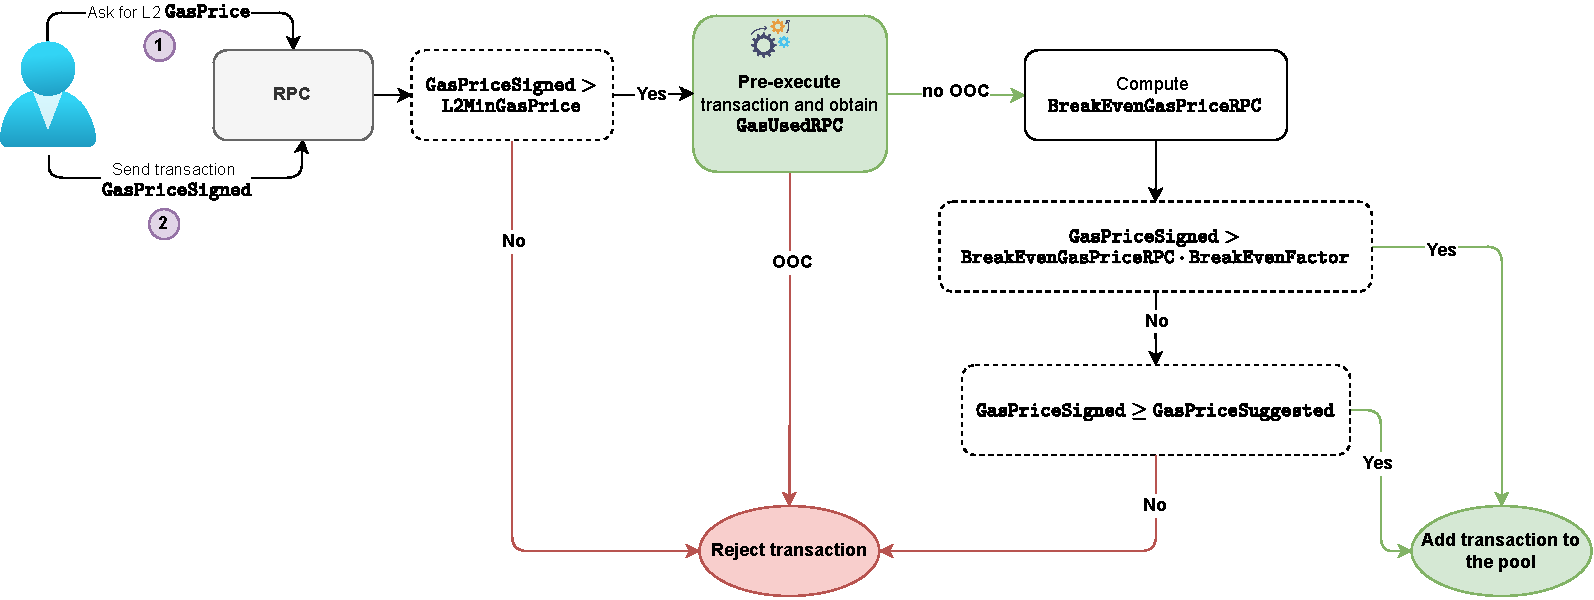
\includegraphics[width=0.9\textwidth]{\zkevmdir/figures/architecture/economics-users-fees/rpc-diagram.drawio}
\caption{Flow of a transaction within the \textbf{RPC} component. As a result of this flow, a transaction can be either included in the \textbf{Pool} for future sequencing or rejected from the network. }
\label{fig:rpc-flow}
\end{figure}

\begin{enumerate}

\item First of all, the users asks to the \textbf{RPC} for the current \texttt{GasPriceSuggested}, which recall is a factor of the current L1 \texttt{GasPrice}. More concretely,
\[
\texttt{GasPriceSuggested} = \texttt{L1GasPrice} \cdot \texttt{SuggestedFactor},
\]
where \texttt{SuggestedFactor} (which is currently of $0.15$) satisfies
\[
\texttt{SuggestedFactor} > \texttt{L1GasPriceFactor}
\]
in order to be able to cover data availability costs. Observe that the suggested gas price varies over time as \texttt{L1GasPrice} also does.

\item Now, the user sends the transaction selecting a \texttt{GasPriceSigned}, the same as in L1. Observe that, from asking for a suggested gas price to sending the transaction has passed some unbounded period of time, where the L1 Gas Price could have increased. Henceforth, rejecting a transaction if $\texttt{GasPriceSigned} < \texttt{GasPriceSuggested}$ does not offer a good user experience. In contrast, we give a margin of $5$ minutes (controlled by the \texttt{MinAllowedGasPriceInterval} parameter). If the signed gas price does not strictly exceed \texttt{MinL2GasPrice}, which is the minumum suggested gas price of $5$ minutes before sending the transaction refreshed every $5$ seconds, called (controlled by the \texttt{IntervalToRefreshGasPrices} parameter),
\[
\texttt{GasPriceSigned} > \texttt{L2MinGasPrice},
\]
we automatically \textbf{reject} the transaction, since it will not be possible to cover costs.

\item If the transaction was not rejected in the previous step, the RPC uses a cloud executor in order to pre-execute the transaction. Observe that this pre-execution is only an estimated execution since the used state root is not the correct one, as the transaction has not been sequenced yet. Recall that once a transaction is added into the \textbf{Pool}, it is mandatory that it is eventually sequenced. Due to this fact, the purpose of this is to filter transactions according and estimate a fair gas price in an early processing stage, to avoid future losses. As a result of this pre-execution it is obtained and estimated amount of used Gas, which will be called \texttt{GasUsedRPC}. If by pre-executing the transaction we run out of counters, we immediately \textbf{reject} the transaction.

\item If the transaction was not reverted due to \textbf{OOC error}, we compute the current break even gas price, which we will call \texttt{BreakEvenGasPriceRPC}. Recall that it depends on the current \texttt{L1GasPrice}, the transaction size, the \texttt{GasUsed RPC} and a parameter \texttt{NetProfit} that is present in order to include the network's profit for the whole transaction's processing.

\item Now, we have two different paths:

\begin{itemize}

\item If the gas price signed by the user at the time of sending the transaction is higher than the \texttt{BreakEvenGasPriceRPC}, increased by a factor $\texttt{BreakEvenFactor} \geq 1$ (and currently set at $1.3$) used to protect the network against bad Gas usage estimations in the RPC
\[
\texttt{GasPriceSigned} > \texttt{BreakEvenGasPriceRPC} \cdot \texttt{BreakEvenFactor}
\]
then the transaction is immediately \textbf{accepted} and stored in the pool.

\item Otherwise, if
\[
\texttt{GasPriceSigned} \leq \texttt{BreakEvenGasPriceRPC} \cdot \texttt{BreakEvenFactor}
\]
we are in dangerous zone because we may be facing losings due high data availability costs or to fluctuation between future computations, so we \textbf{should reject} the transaction. However, we are currently not directly rejecting transactions in this case.

\end{itemize}

\item In the later case, we check if the gas price signed with the transaction exceeds the current suggested gas price:
\[
\texttt{GasPriceSigned} \geq \texttt{GasPriceSuggested}.
\]
In this case, we take the risk of possible losses, sponsoring the difference if necessary and we introduce the transaction into the \textbf{Pool}. However, if $\texttt{GasPriceSigned} < \texttt{GasPriceSuggested}$ we assume that is highly probable that we face losing and we immediately reject the transaction.

\end{enumerate}


\paragraph*{Final Considerations}

It is important to remark that, as we have said before, once a transaction is included into the pool, we should actually sequence it, that is, we should include it into a block. Hence, if something goes bad in later steps and the gas consumption deviates significantly from the initial estimate, we risk incurring losses with no means to rectify the situation. On the contrary, if the process goes as estimated and the consumed gas is similar to the estimated one, we can reward the user by modifying the previously introduced \texttt{effectivePercentage}. Additionally, it’s important to observe that, among all the transactions stored in the Pool, the ones prioritized at the time of sequencing are the ones with higher \texttt{effectiveGasPrice}, due to the prioritization introduced with \texttt{ratioPriority}. Observe that \texttt{effectiveGasPrice} \textbf{is not} computed in the \textbf{RPC} but in the \textbf{Sequencer}, so it possible that the suggested gas price at this moment differs from the suggested one when user sent the transaction.



\subsection{Numerical Example: RPC Flow} \label{sec:numerical-example-rpc}

Let us continue the numerical example that has been carried during the whole document. In Figure \ref{fig:numerical-example-rpc} we represent, at the top of the timeline, the current \texttt{L1GasPrice} and, at the bottom, the associated $\texttt{GasPriceSuggested} = 0.15 \cdot \texttt{L1GasPrice}$.

\begin{figure}[H]
\centering
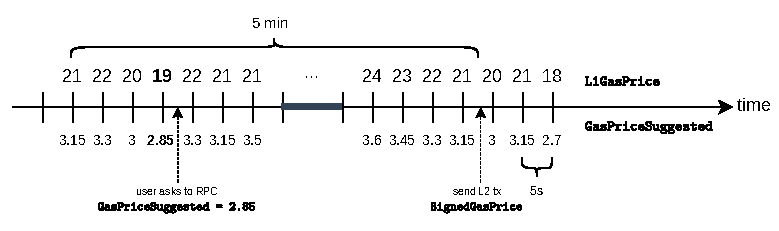
\includegraphics[width=0.9\textwidth]{\zkevmdir/figures/architecture/economics-users-fees/example-minimum-gas-price.drawio}
\caption{Timeline displaying the current \texttt{L1GasPrice} and its associated suggested gas price. }
\label{fig:numerical-example-rpc}
\end{figure}

\begin{enumerate}

\item At the time marked with the left arrow, the user queries the RPC for the suggested gas price when \texttt{L1GasPrice} is $19$, and receives a as response the value of $2.85$ GWei/Gas:
\[
\texttt{GasPriceSuggested} = 0.15 \cdot 19 = 2.85 \text{ GWei/Gas}.
\]

\item Let us suppose that the users sends a transaction signed with a gas price of $3$
\[
\texttt{GasPriceSigned} = 3.
\]
Observe that the signed gas price is strictly lower than the current suggested gas price, which is $3.15 = 21 \cdot 0.15$. However, recall that at this precise step we are allowing all the transactions with a signed gas price exceeding the minimum suggested gas price $5$ minutes before sending the transaction refreshed every $5$ seconds. Henceforth, since
\[
\texttt{GasPriceSigned} = 3 > 2.85 = \texttt{L2MinGasPrice},
\]
we accept the transaction at this point.

\item At this point, the RPC asks for a pre-execution, getting an estimation for the gas used, computed with a state root that will differ from the one used when sequencing the transaction. In this case, we get a gas used estimation of
\[
\texttt{GasUsedRPC} = 60,000 \text{ Gas},
\]
without running out of counters.

\item Since we have not run out of counters, we compute \texttt{BreakEvenGasPriceRPC} supposing same transaction sizes as before and getting
\[
\texttt{BreakEvenGasPriceRPC} = 2.52 \text{ GWei/Gas}.
\]

\item Notice that, in this particular scenario, despite having
\[
\texttt{GasPriceSigned} < \texttt{BreakEvenGasPriceRPC},
\]
the introduction of the \texttt{BreakEvenFactor} (which acts as a protective measure as previously discussed) results in the next check failure:
\[
\texttt{GasPriceSigned} < 3.276 = 2.52 \cdot 1.3 = \texttt{BreakEvenGasPrice} \cdot \texttt{BreakEvenFactor}.
\]

\item However, recall that but we are currently sponsoring and accepting all transactions as long as
\[
\texttt{GasPriceSigned} = 3 \geq 2.85 = \texttt{GasPriceSuggested},
\]
which is the current case. Henceforth, we accept the transaction and store it into the \textbf{Pool}.

\end{enumerate}



\subsection{Sequencer Flow}

The \textbf{Sequencer} is the zkEVM component that is responsible for fetching transactions from the \textbf{Pool} and assembling some of them into a \textbf{batch}. The sequencer submits a sequence of batches to the L1 which will be then proved by the \textbf{Aggregator}. In Figure \ref{fig:sequencer-flow}, the transaction progression within the \textbf{Sequencer} component is shown, starting from the moment that a transaction is fetched from the \textbf{Pool} until it is executed by the \textbf{Executor}. Let's examine the Figure \ref{fig:sequencer-flow} in detail.

\begin{figure}[H]
\centering
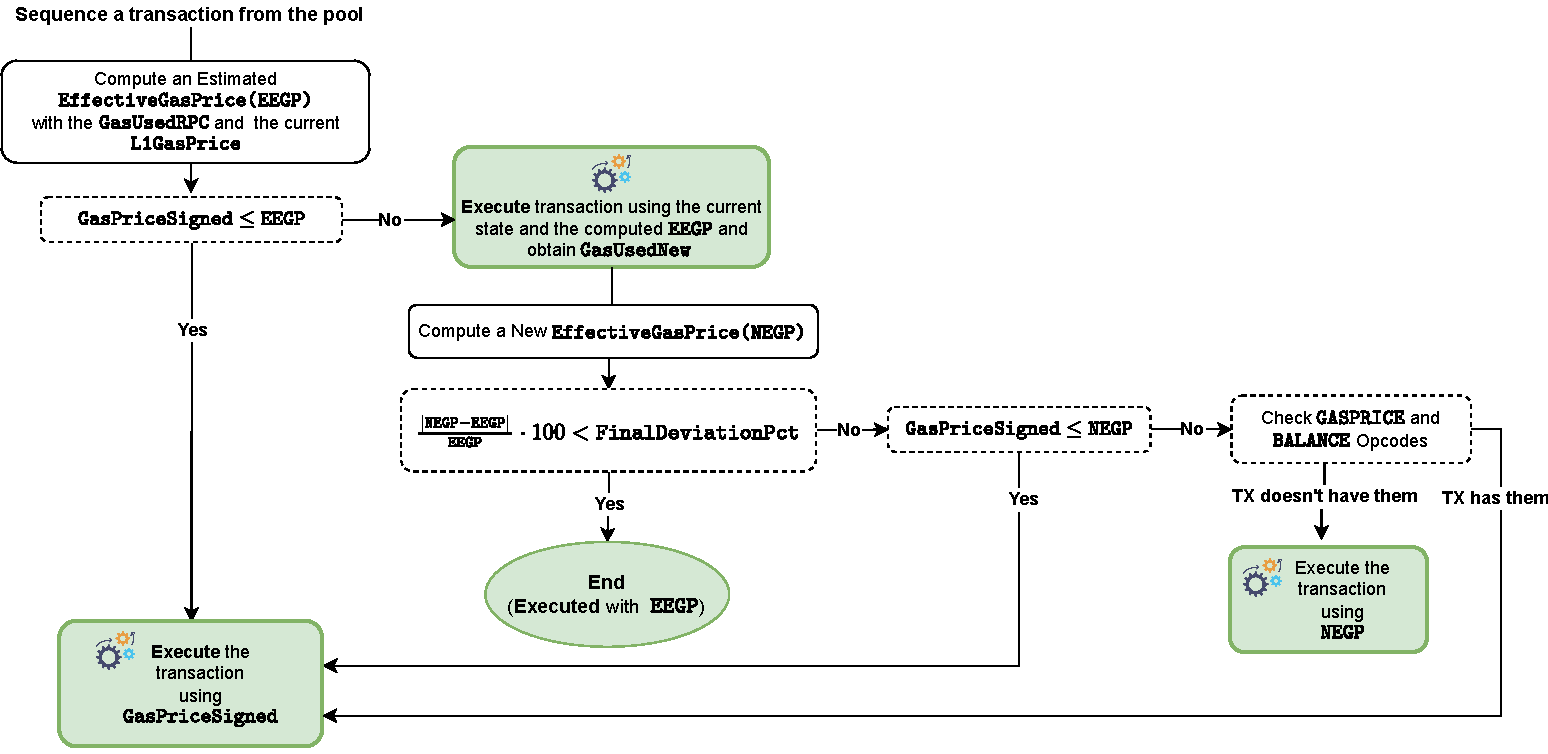
\includegraphics[width=0.9\textwidth]{\zkevmdir/figures/architecture/economics-users-fees/sequencer-diagram.drawio}
\caption{Flow of a transaction within the \textbf{Sequencer} component. Observe that we can not reject transactions at this point, so all of them should be included in the L1 State. }
\label{fig:sequencer-flow}
\end{figure}

\begin{enumerate}

\item The \textbf{Sequencer} computes the estimated \texttt{EffectiveGasPrice} (which we will call \texttt{EEGP}) using the \texttt{GasUsedRPC} obtained in the \textbf{RPC} pre-execution using a previous state root (which has now changed) and the current \texttt{L1GasPrice} (which also may differ from the one used when sending the transaction to the \textbf{RPC}) for all the transactions stored in the \textbf{Pool} and sequence the one having higher \texttt{EEGP}. It is important to note that this is done in this precise order. We could have calculated the \texttt{EEGP} just before storing the transactions in the \textbf{Pool} and sorting it by \texttt{EEGP}, but this would not yield the same result because the \texttt{L1GasPrice} at that moment is different from the one at the time of sequencing a transaction, potentially changing the \texttt{EEGP} as well as the prioritization order of transactions.

\item At this point, we have two options:

\begin{itemize}

\item If $\texttt{GasPriceSigned} \leq \texttt{EEGP}$, even with only an estimated effective gas price, there is a significant risk of loss. In such cases, we opt not to further adjust the gas price in order to reduce the number of executions needed to do so. Henceforth, the user is charged the full \texttt{GasPriceSigned}, so the \textbf{Executor} will execute the transaction using it, concluding the sequencing process.

\item Conversely, if $\texttt{GasPriceSigned} > \texttt{EEGP}$, there is a potential room for further adjustment for the gas price that will be charged to the user.

\end{itemize}

\item In the previous case, it is necessary to compute a more precise effective gas price based on the accurate amount of gas, denoted as \texttt{GasUsedNew}, obtained during the transaction's execution using the correct state root at the sequencing time (which was not known earlier for straightforward reasons). Henceforth, the \textbf{Executor} executes the transaction using \texttt{EEGP}, obtaining \texttt{GasUsedNew} which the sequencer utilizes to compute a new effective gas price referred to as \texttt{NEGP}.

\item We have to paths:

\begin{itemize}

\item If the percentage deviation between \texttt{EEGP} and \texttt{NEGP} is higher than a fixed deviation parameter \texttt{FinalDeviationPct} (which is $10$ in the actual configuration), that is
\[
\frac{\vert \texttt{NEGP} - \texttt{EEGP} \vert}{\texttt{EEGP}} \cdot 100 < \texttt{FinalDeviationParameter},
\]
indicates that there is minimal distinction between charging the user with \texttt{NEGP} compared to \texttt{EEGP}. Therefore, despite potential (but quite small) losses to the network or the user, we end up the flow just to avoid re-executions and save execution resources and we charge the user with \texttt{EEGP}.

\item On the contrary, if the percentage deviation equals or exceeds the deviation parameter
\[
\frac{\vert \texttt{NEGP} - \texttt{EEGP} \vert}{\texttt{EEGP}} \cdot 100 \geq \texttt{FinalDeviationParameter},
\]
there is a big difference between executions and we may better adjust gas price to potential (and quite big) losses to the network or the user.


\end{itemize}

\item In the later case, two options arise:

\begin{itemize}

\item If the gas price signed is less or equal than the accurate effective gas price computed with the correct state root
\[
\texttt{GasPriceSigned} \leq \texttt{NEGP},
\]
the network suffers again a risk of loss. Henceforth, the user is charged the full \texttt{GasPriceSigned}, so the \textbf{Executor} will execute the transaction using it, concluding the sequencing process.

\item Otherwise, if
\[
\texttt{GasPriceSigned} > \texttt{NEGP},
\]
means that we have margin to adjust the gas price that is charged to the user. However, in order to save executions and end up the adjustment process in this iteration, we will conclude the flow using a trick explained in the next point.

\end{itemize}

\item In the later case, we check if the transaction processing includes the two opcodes that use the gas price:

\begin{itemize}[-]

\item The \texttt{GASPRICE} opcode.

\item The \texttt{BALANCE} opcode from the source address.

\end{itemize}

We have two cases:

\begin{itemize}

\item If the transaction contains the aforementioned opcodes, we impose a penalty on the user for security reasons. In such cases, we simply proceed with executing the transaction using the entire \texttt{GasPriceSigned} to minimize potential losses and conclude the flow, as mentioned earlier. This precaution is employed to mitigate potential vulnerabilities in deployed Smart Contracts, that arise from creating a specific condition based on the gas price, for example, to manipulate execution costs.

\item If the transaction does not make use of the gas price-related opcodes, the \textbf{Executor} executes the transaction with the more adjusted gas price up to this point which is \texttt{NEGP} and end up the sequencing process.

\end{itemize}

\end{enumerate}



\subsection{Numerical Example: Sequencer Flow}


Let us continue the numerical example that has been carried during the whole document. In Figure \ref{fig:numerical-example-rpc} we represent, at the top of the timeline, the current \texttt{L1GasPrice} and, at the bottom, the associated $\texttt{GasPriceSuggested} = 0.15 \cdot \texttt{L1GasPrice}$ at the time of sequencing the transaction. Recall that in Section \ref{sec:numerical-example-rpc} we end up computing the \texttt{BreakEvenGasPriceRPC} of $2.52$ GWei/Gas.


\begin{figure}[H]
\centering
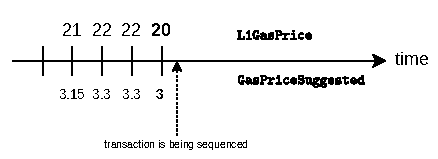
\includegraphics[width=0.7\textwidth]{\zkevmdir/figures/architecture/economics-users-fees/numerical-example-sequencer.drawio}
\caption{Timeline displaying the current \texttt{L1GasPrice} and its associated suggested gas price at the time of sequencing the transaction. }
\label{fig:numerical-example-sequencer}
\end{figure}


\begin{enumerate}

\item Imagine that the user signed a gas price $3.3$ GWei/Gas. As illustrated in Figure \ref{fig:numerical-example-sequencer}, the network recommends a gas price of $3$ at the sequencing moment, equivalent to an L1 gas price of $20$. This results in an \texttt{EEGP} of
\[
\texttt{EEGP} = 2.722 \text{ GWei/Gas},
\]
where the $10$\% increase attributed to the prioritization carried out by \texttt{PriorityRatio} set at $0.1$.

\item Since the signed gas price is bigger than the estimated effective gas price
\[
\texttt{GasPriceSigned} = 3.3 > 2.772 = \texttt{EEGP},
\]
we execute the transaction using the current (and correct) state and the computed \texttt{EEGP} in order to obtain an accurate measure of the Gas used, which we call \texttt{GasUsedNew}. Suppose that, in this case, we obtain
\[
\texttt{GasUsedNew} = 95,000 \text{ Gas},
\]
which is bigger than the estimated gas of $60,000$ at the \textbf{RPC} pre-execution.

\item By using \texttt{GasUsedNew}, we can compute and adjusted effective gas price called \texttt{NEGP} as follows:
\begin{gather*}
\texttt{TxCostNew} = (200 \cdot 16 + 100 \cdot 4) \cdot 20 + 95,000 \cdot 20 \cdot 0.04 = 148,000 \text{ GWei}, \\
\texttt{BreakEvenGasPriceNew} = \frac{148,000}{95,000} \cdot 1.2 = 1.869 \text{ GWei/Gas}, \\
\texttt{NEGP} = 1.869 \cdot 1.1 = 2.056 \text{ GWei/Gas}.
\end{gather*}

Observe that the transaction cost is way higher than the estimated one of $126,000$ even when the L1 Gas Price has decreased from $21$ to $20$ due to a huge increase in Gas.

\item Observe that there is a significative deviation between both effective gas prices:
\[
\frac{\vert \texttt{NEGP} - \texttt{EEGP} \vert}{\texttt{EEGP}} \cdot 100 = 25.82 > 10.
\]
This deviation penalizes the user a lot since
\[
\texttt{GasPriceSigned} = 3 > 2.52 = \texttt{EEGP} \gg 2.056 = \texttt{NEGP},
\]
so we try to charge \texttt{NEGP} to the user to further adjust the gas price.

\item In this case, suppose that the transaction does not have neither \texttt{GASPRICE} nor \texttt{BALANCE} (from the source address) opcodes, so we will execute the transaction with
\[
\texttt{GasPriceFinal} = \texttt{NEGP} = 2.056 \text{ GWei/Gas}.
\]
Observe that \texttt{GasUsedFinal} should be the same as \texttt{GasUsedNew} $= 95,000$. We can now compute \texttt{EffectivePercentage} and \texttt{EffectivePercentageByte} as follows:
\begin{gather*}
\texttt{EffectivePercentage} = \frac{\texttt{GasPriceFinal}}{\texttt{GasPriceSigned}} = \frac{2.056}{3.3} = 0.623. \\
\texttt{EffectivePercentageByte} = \texttt{EffectivePercentage} \cdot 256  - 1 = 148.
\end{gather*}
Observe that the user has been charged with the $62.3$\% of the gas price he/she signed at the time of sending the transaction.

\end{enumerate}

%\newpage
%\bibliographystyle{alpha}
%\bibliography{../bib/bibliography}

\newpage
\appendix

\end{document}